\chapter{Pythia}
Pythia is a general-purpose event generator. It is extensively used for studying physics at LHC. At the beginning the code was written in \verb+Fortran 77+, recently it has been moved to \verb!C++!. The latest version of Pythia (8.1) was released in 2007, which is written in \verb!c++!  \citep{Buckley:2011ms}. 

In general Pythia performs on idea of the program designed here for the parton shower. However, it accounts for more of the underlying physics,that we have not covered in our model. Such  as the quark flavour or in general the type of the particle which is splitting.  

\section{FastJet} 

\verb+FastJet+ is an analysis tools, it written in \verb!C++!. It includes efficient implementation of all widely used sequential recombination jet algorithms. In the case of jet clustering, the working principle is the same as the algorithm that we implemented in chapter 4, but it is much faster \citep{Buckley:2011ms}. 

In our work we generated 1000 events using Pythia 8.1 and analysed them using \verb+FastJet+ using the configuration $dijet$, which is the a simulation of a collision that produces two particles. 

We extracted the same  observables as in \ref{nofcon}, \ref{nofjet} and \ref{pseudomass}  the pseudo-mass, the number of constituents in the jet with highest energy and the number of jet observables. Here the value of the parameter $R$ is set to 1.
\begin{figure}[hbtp]
\centering
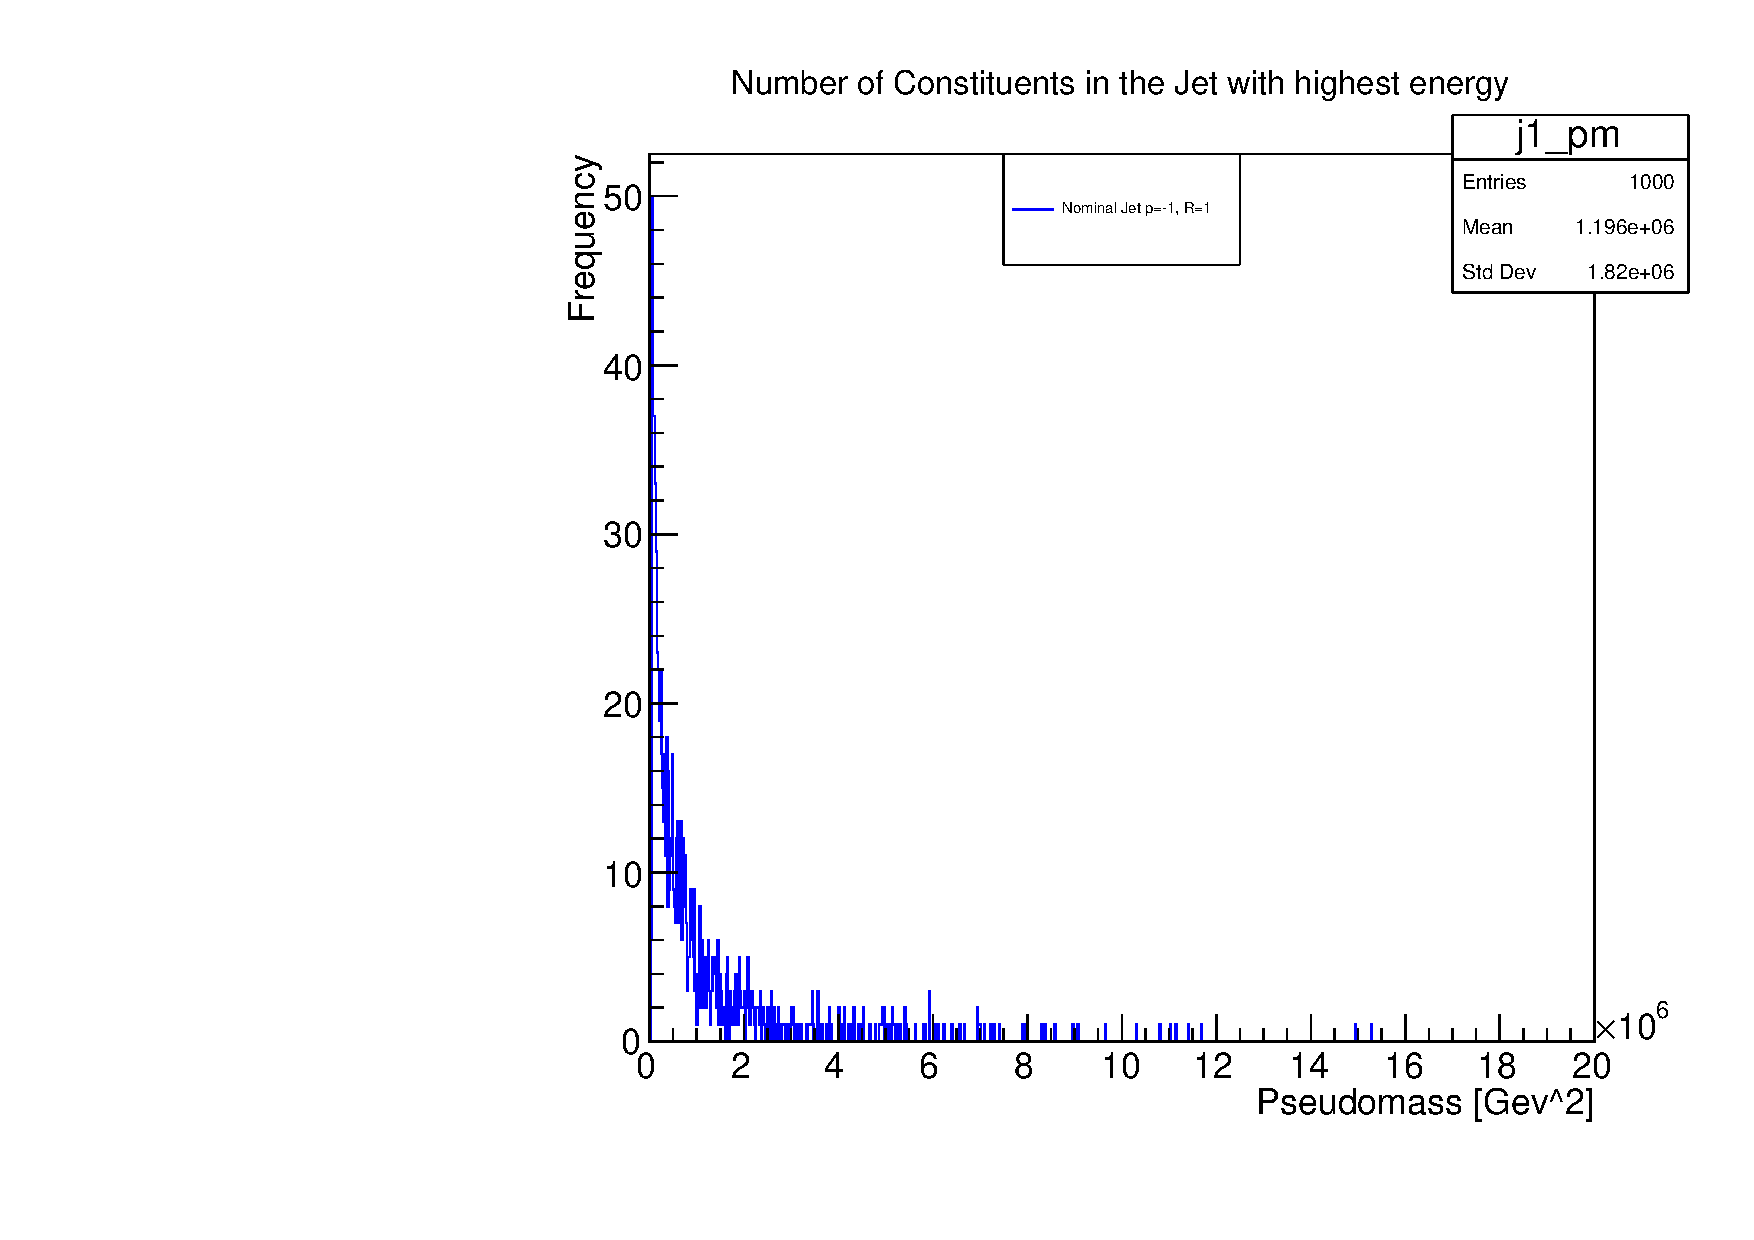
\includegraphics[scale=.7]{images/myplot1.pdf}
\caption{A histogram of the pseudo-mass of a jet observable obtained from analysing 1000 events. $R$ is chosen to be 1.}
\end{figure}



\begin{figure}[hbtp]
\centering
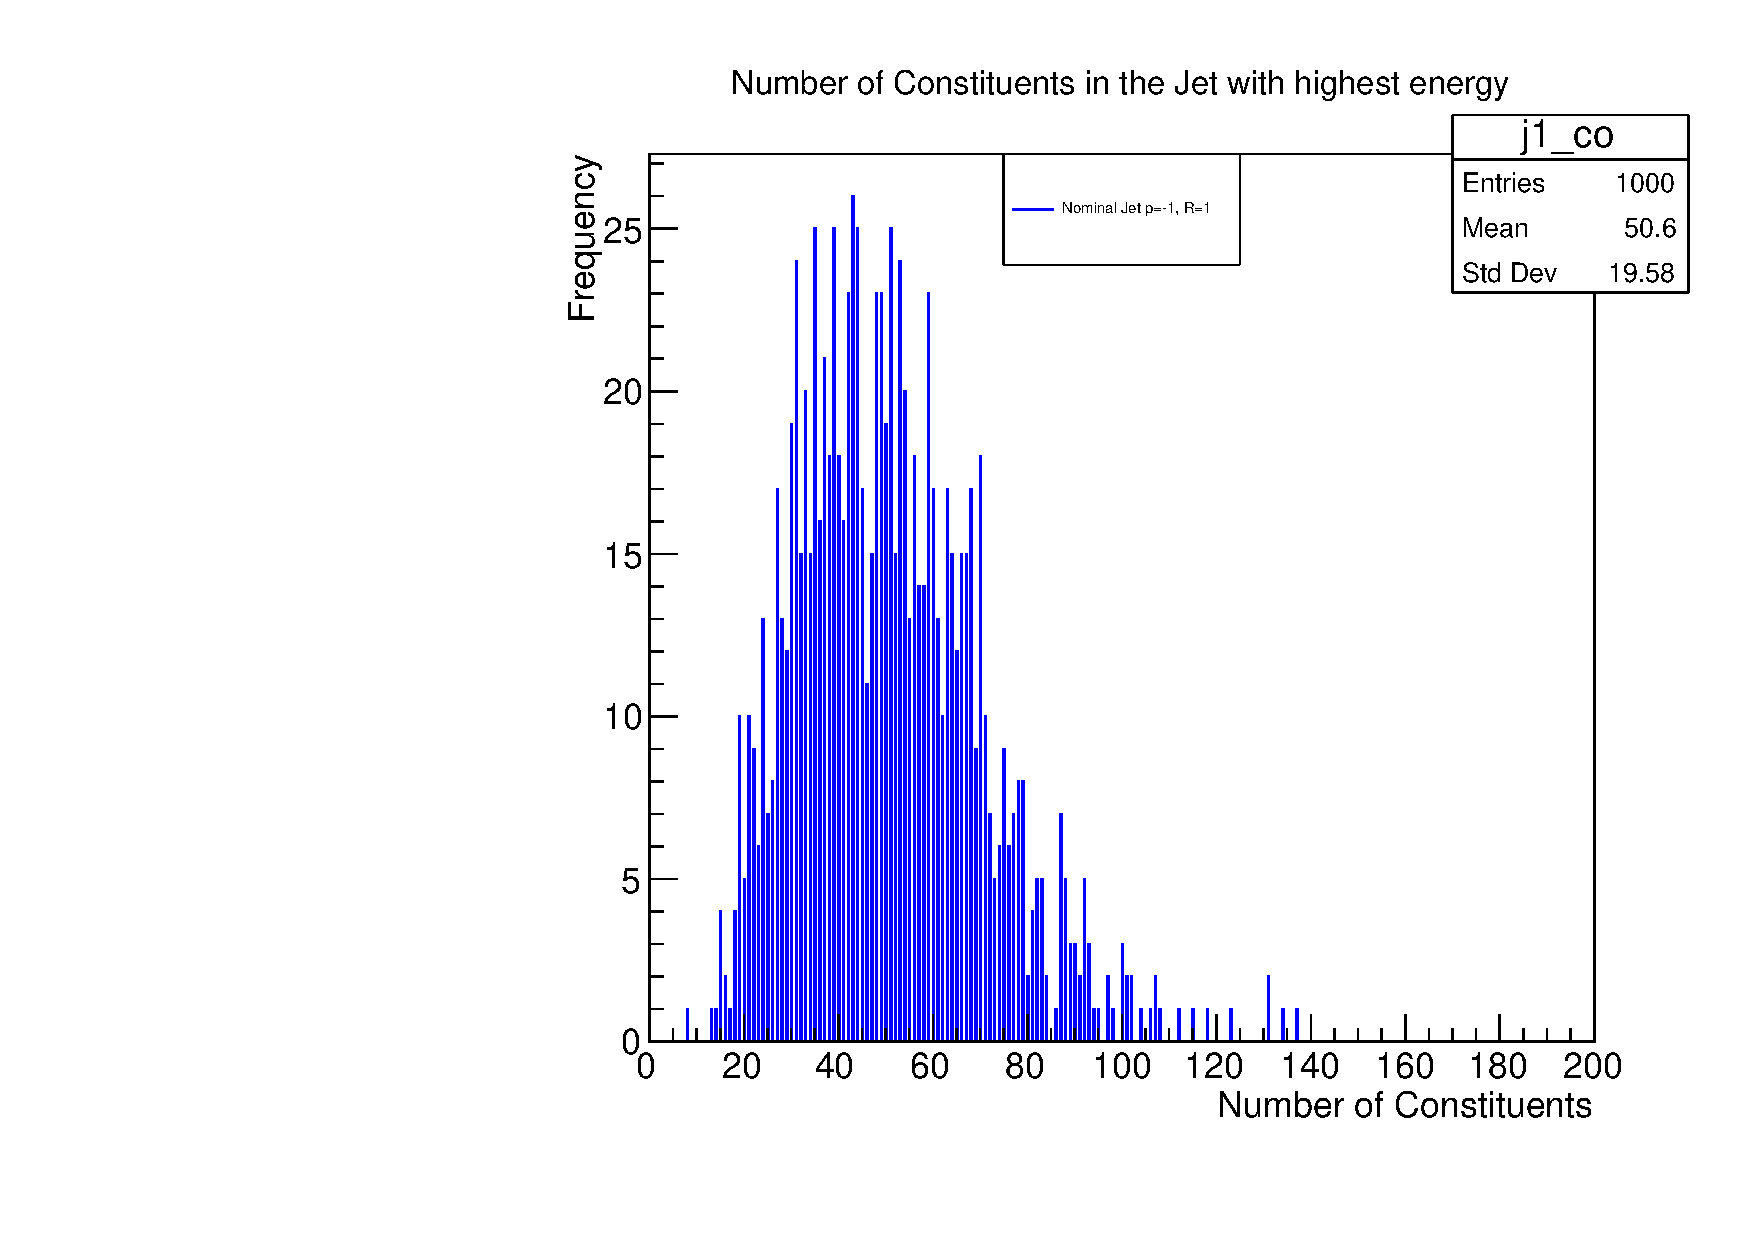
\includegraphics[scale=.7]{images/myplot3.pdf}
\caption{A histogram of the number of constituents in the jet with highest energy obtained from analysing 1000 events.}
\end{figure}

 
\begin{figure}[hbtp]
\centering
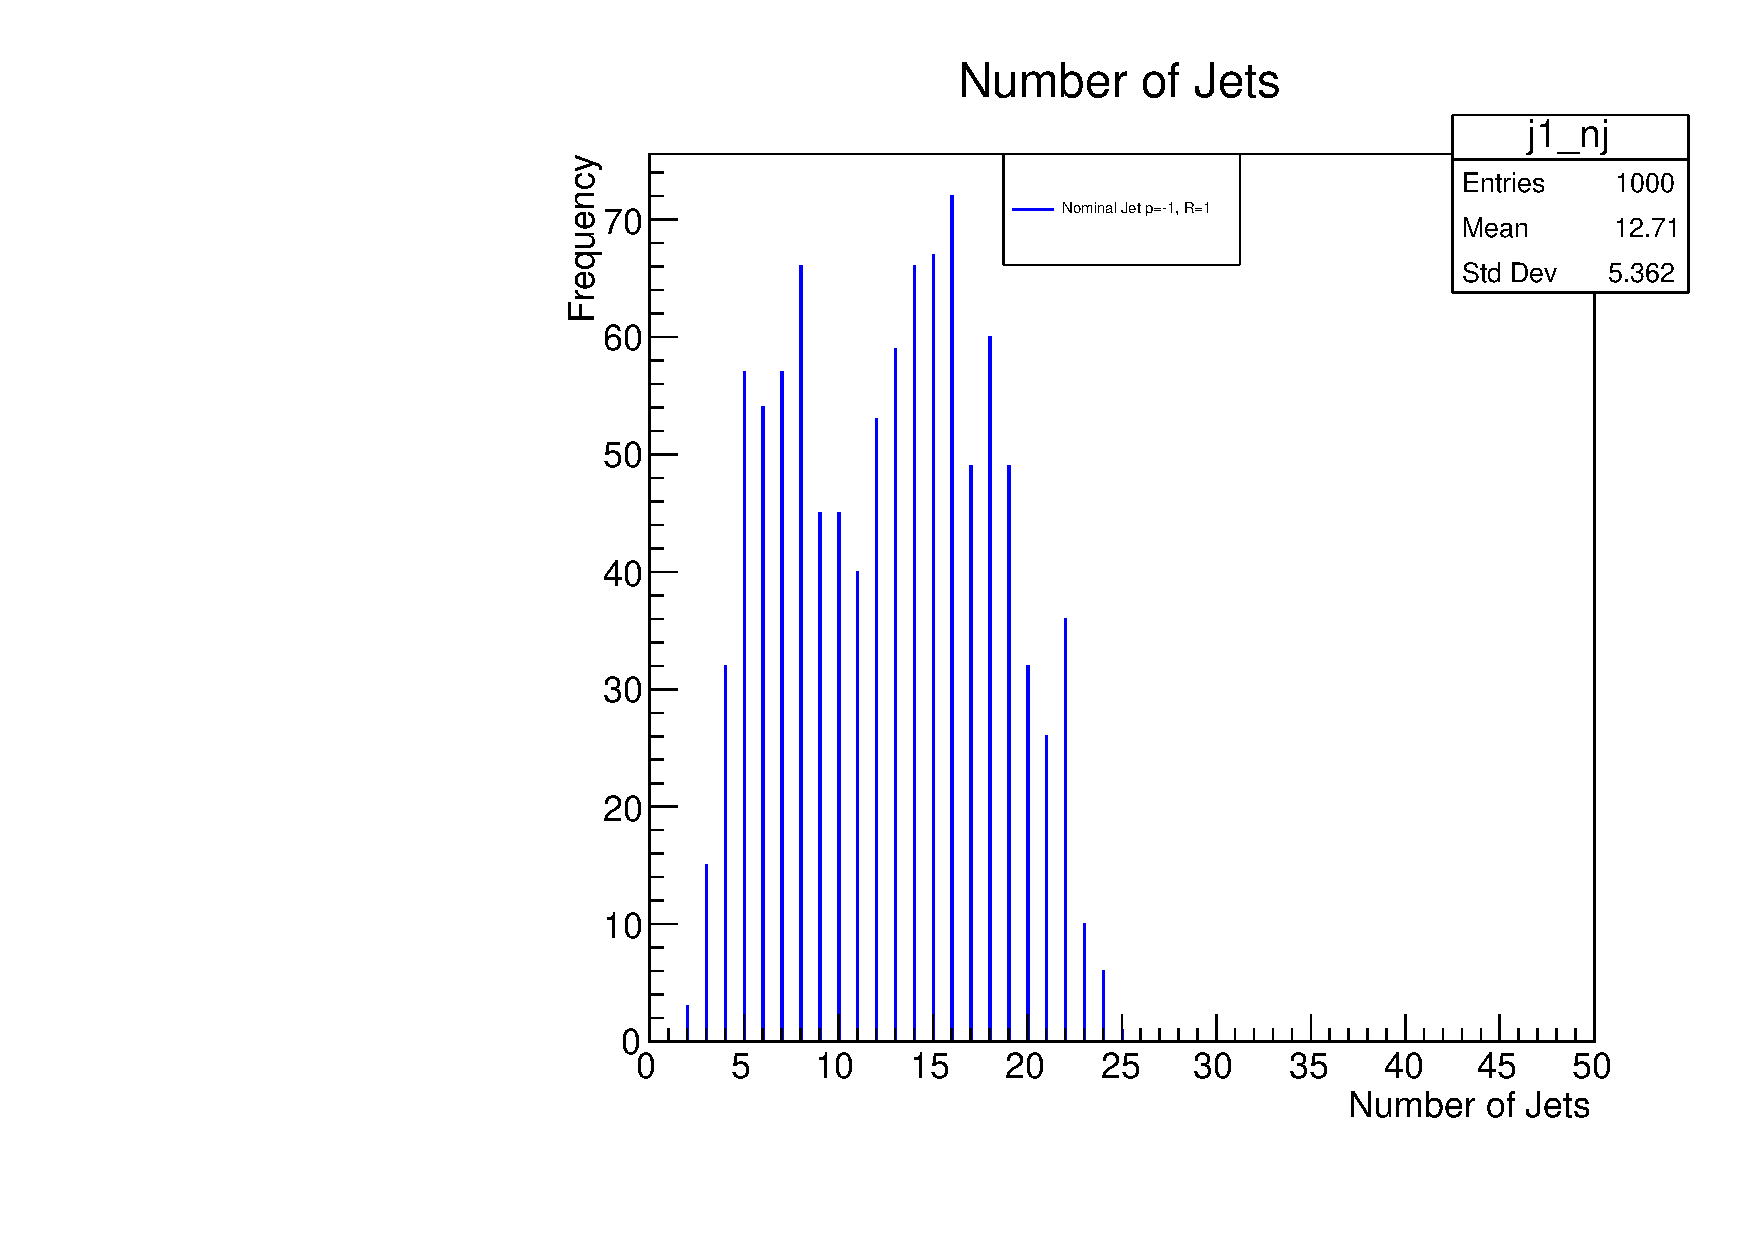
\includegraphics[scale=.7]{images/myplot2.pdf}
\caption{A histogram of the number of jet obtained analysing from 1000 events.}
\end{figure}

%\begin{figure}[hbtp]
%\centering
%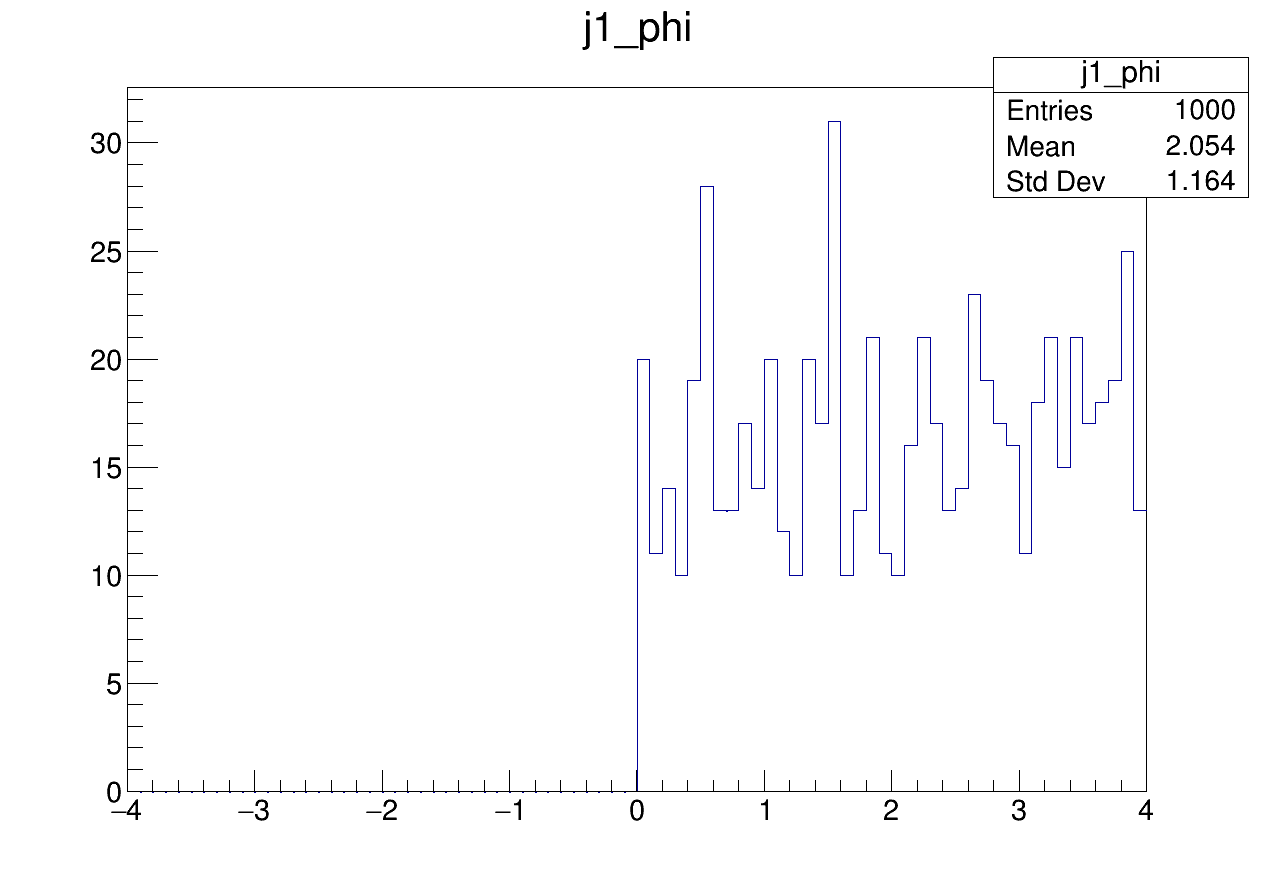
\includegraphics[scale=.4]{images/phi.png}
%\caption{The Azimuth distance.  }
%\end{figure}
%
%\begin{figure}[hbtp]
%\centering
%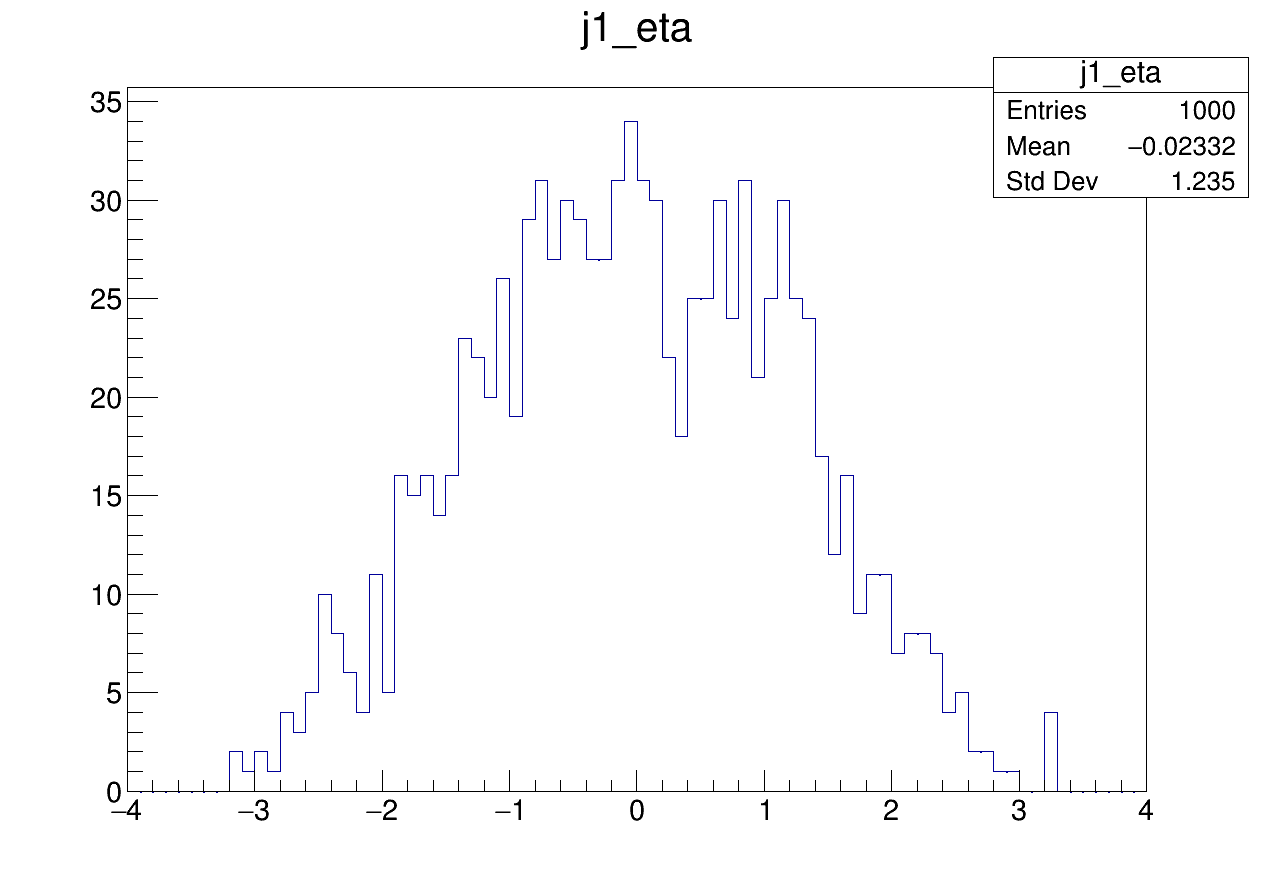
\includegraphics[scale=.3]{images/eta.png}
%\caption{The pseudo-rapidity}
%\end{figure}

      